\chapter{Test of the frequency and time domain response of the effects}\label{chap:effect_test_response}

Responses of the effects to waves are being tested to verify if they are well operating by comparing the shape to a MATLAB simulation. 

\section{Material and Setup}

The use material to perform the test is:

\begin{itemize}
	\item A computer with MATLAB, Waveforms 2015 and Code Composer
	\item Wave Generator Digilent Analog Discovery 2
	\item The DSP TMS320C5515
	\item Wires
\end{itemize}

The wave generator is connected to the stereo input of the DSP. Two scopes are used, one connected on the input and the other one on the output. The computer is used to load the compiled code on the DSP, inspect what is on the scopes using Waveforms 2015. 
Measuring the response in frequency domain or time domain depends on the effect, time domain may be useful in some cases and not in the others. 
The step after is to compare it with the simulation on MATLAB and see whether the shapes are similar enough to conclude that the effect is working well on the DSP. 

\begin{figure}[hbt]
  \begin{picture}(0,0)%
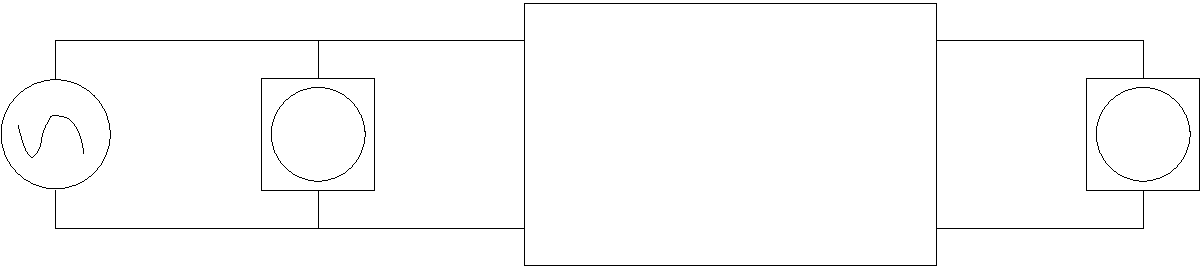
\includegraphics[width=1\textwidth]{effect_test_set.pdf}%
\end{picture}%
\setlength{\unitlength}{3947sp}%
%
\begingroup\makeatletter\ifx\SetFigFont\undefined%
\gdef\SetFigFont#1#2#3#4#5{%
  \reset@font\fontsize{#1}{#2pt}%
  \fontfamily{#3}\fontseries{#4}\fontshape{#5}%
  \selectfont}%
\fi\endgroup%
\begin{picture}(9607,2124)(2406,-5173)
\put(6001,-4336){\makebox(0,0)[lb]{\smash{{\SetFigFont{12}{14.4}{\rmdefault}{\mddefault}{\updefault}{\color[rgb]{0,0,0}DSP}%
}}}}
\end{picture}%
\caption{Figure showing the test setup}
\end{figure}


\section{Results}

Results for each effect will be presented in a different subsection. 

\subsection{Results for the Reverb Effect}






\subsection{Results for the Equalizer Effect}


\subsection{Results for the Flanger Effect}